\documentclass{article}
\usepackage[utf8]{inputenc}
\usepackage{amsmath}
\usepackage{pgfplots}
\pgfplotsset{compat=newest}
\usepackage{tikz}
\usetikzlibrary{plotmarks}

\begin{document}

\begin{figure}[h]
    \centering
    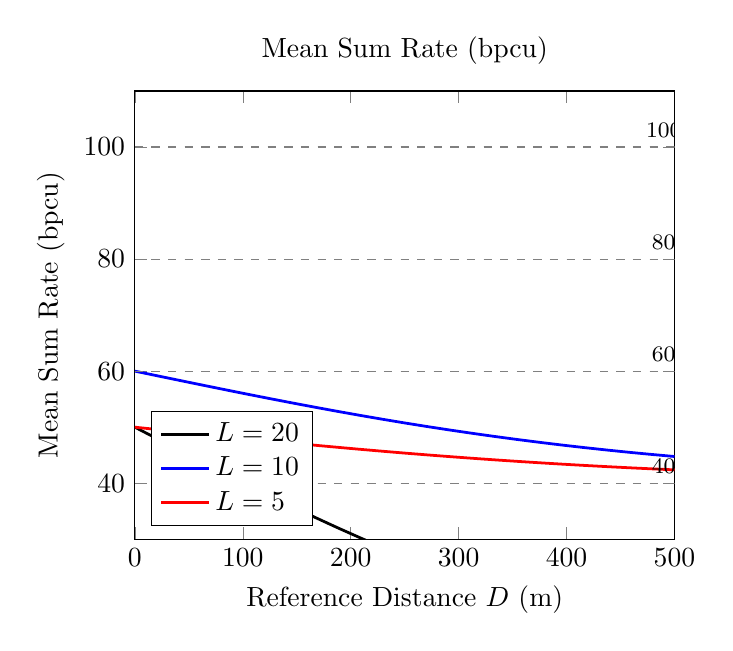
\begin{tikzpicture}
        \begin{axis}[
            title={Mean Sum Rate (\textnormal{bpcu})},
            xlabel={Reference Distance $D$ (m)},
            ylabel={Mean Sum Rate (bpcu)},
            legend pos=south west,
            ymajorgrids=true,
            grid style=dashed,
            ymin=30, ymax=110, % Adjusted for better visibility
            xmin=0, xmax=500,
            legend entries={$L=20$, $L=10$, $L=5$},
            legend cell align=left, % Align legend entries left
            legend style={cells={align=center}},
            ]
            \addplot[
                domain=0:500, 
                color=black,
                mark size=2pt,
                line width=1.0pt,
                ]
                {100 - 100/(1 + exp(-0.004*x))};
            \addlegendentry{$L=20$};
            
            \addplot[
                domain=0:500, 
                color=blue,
                mark size=2pt,
                line width=1.0pt,
                ]
                {80 - 40/(1 + exp(-0.004*x))};
            \addlegendentry{$L=10$};
            
            \addplot[
                domain=0:500, 
                color=red,
                mark size=2pt,
                line width=1.0pt,
                ]
                {60 - 20/(1 + exp(-0.004*x))};
            \addlegendentry{$L=5$};
            
            % Horizontal dashed lines representing FC operation
            \addplot[
                domain=0:500, 
                color=gray,
                dashed,
                ]
                {100};
            \node at (490,100) [above] {\footnotesize 100};
            
            \addplot[
                domain=0:500, 
                color=gray,
                dashed,
                ]
                {80};
            \node at (490,80) [above] {\footnotesize 80};
            
            \addplot[
                domain=0:500, 
                color=gray,
                dashed,
                ]
                {60};
            \node at (490,60) [above] {\footnotesize 60};
            
            \addplot[
                domain=0:500, 
                color=gray,
                dashed,
                ]
                {40};
            \node at (490,40) [above] {\footnotesize 40};
        \end{axis}
    \end{tikzpicture}
    \caption{Sum rate of PCNC scheme with respect to the reference distance $D$. The dashed lines represent the sum rates of the FC operation. Parameters for the plot: $M=5$, $K=5$, $N=2$, and $d_{kc} = 2 \;\forall k,c$.}
    \label{fig:sum_rate_with_D}
\end{figure}

\end{document}